\begin{frame}{Track Reconstruction Efficiency for ALMA9}
    \begin{itemize}
        \item Objective was to validate the track reconstruction for Dark Photon samples in ALMA9.
        \item Dark Photon samples have closely separated tracking making reconstruction difficult.
        \item Idea was to see if ALMA9 ``performs'' better than CENTOS7 
        \item Sined already worked out the studies on single muon 
        \item Ansh started out looking at the Analysis Cutflows
        \item Hoping to present on Monday in the Offline Software Meeting
    \end{itemize}
\end{frame}


\begin{frame}{DarkPhoton Tracking CutFlow}
    \begin{table}[h]
        \centering
        \resizebox{\linewidth}{!}{ 
            \begin{tabular}{lccccccccc}
                \toprule
                \multirow{2}{*}{Selection} & \multicolumn{4}{c}{ALMA9} & \multicolumn{4}{c}{CENTOS7} & \multirow{2}{*}{$\Delta$Eff.} \\
                \cmidrule(lr){2-5} \cmidrule(lr){6-9}
                & Pass & All & Eff. & Cum. Eff.
                & Pass & All & Eff. & Cum. Eff. \\
                \midrule
                $\geq$1 LongTracks & 56989 & 60000 & 94.98 & 94.98  & 56002 & 60000 & 93.34 & 93.34 & 1.64 \\
                $\geq$2 LongTracks & 46416 & 56989 & 81.45 & 77.36  & 45210 & 56002 & 80.73 & 75.35 & 0.72 \\
                 =2 LongTracks & 37807 & 46416 & 81.45 & 63.01  & 36746 & 45210 & 81.28 & 61.24 & 0.17 \\
                 \textcolor{red}{\textbf{Opposite Charge}} & 32427 & 37807 & 85.77 & 54.04  & 30375 & 36746 & 82.66 & 50.62 & \textcolor{red}{\textbf{3.11}}\\
                MaxRadius $<$ 100 & 31489 & 32427 & 97.11 & 52.48  & 29520 & 30375 & 97.19 & 49.20 & -0.08 \\
                \midrule
                \multicolumn{10}{c}{goodTrack Cuts}\\
                \midrule
                $\geq$ 7 Layers & 31435 & 31489 & 99.83  & 52.39  & 29472 & 29520 & 99.84  & 49.12 & -0.01 \\
                \textcolor{red}{\textbf{$\chi^2$/DoF $<$ 25}} & 31121 & 31435 & 99.00  & 51.87  & 27710 & 29472 & 94.02  & 46.18& \textcolor{red}{\textbf{4.98}} \\
                $\geq$ 7 DoF & 31115 & 31121 & 99.98  & 51.86    & 27706 & 27710 & 99.99  & 46.18 & -0.01\\
                \bottomrule
            \end{tabular}
        }
        \caption{Comparison of efficiency and cumulative efficiency for ALMA9 and CENTOS7.\\Note: The Cutflow is at an Event Level (not track level), thus the conditions have to met by all tracks in the event.}
        \label{tab:efficiency_comparison}
    \end{table}
    \begin{itemize}
        \scriptsize
        \item Highest improvment in goodTrack Cut of $\chi^2$/DoF $<$ 25
        \item Better ChargeID in ALMA9?
    \end{itemize}    
\end{frame}

\begin{frame}{Track Efficiency for ALMA9  -- Some Plots}
    \begin{itemize}
        \item Had an existing overlay study on Track Reconstruction 
    \end{itemize}
    \vspace{-0.5cm}
    \begin{columns}
        \begin{column}{0.5 \textwidth}
            \begin{figure}
                \centering
                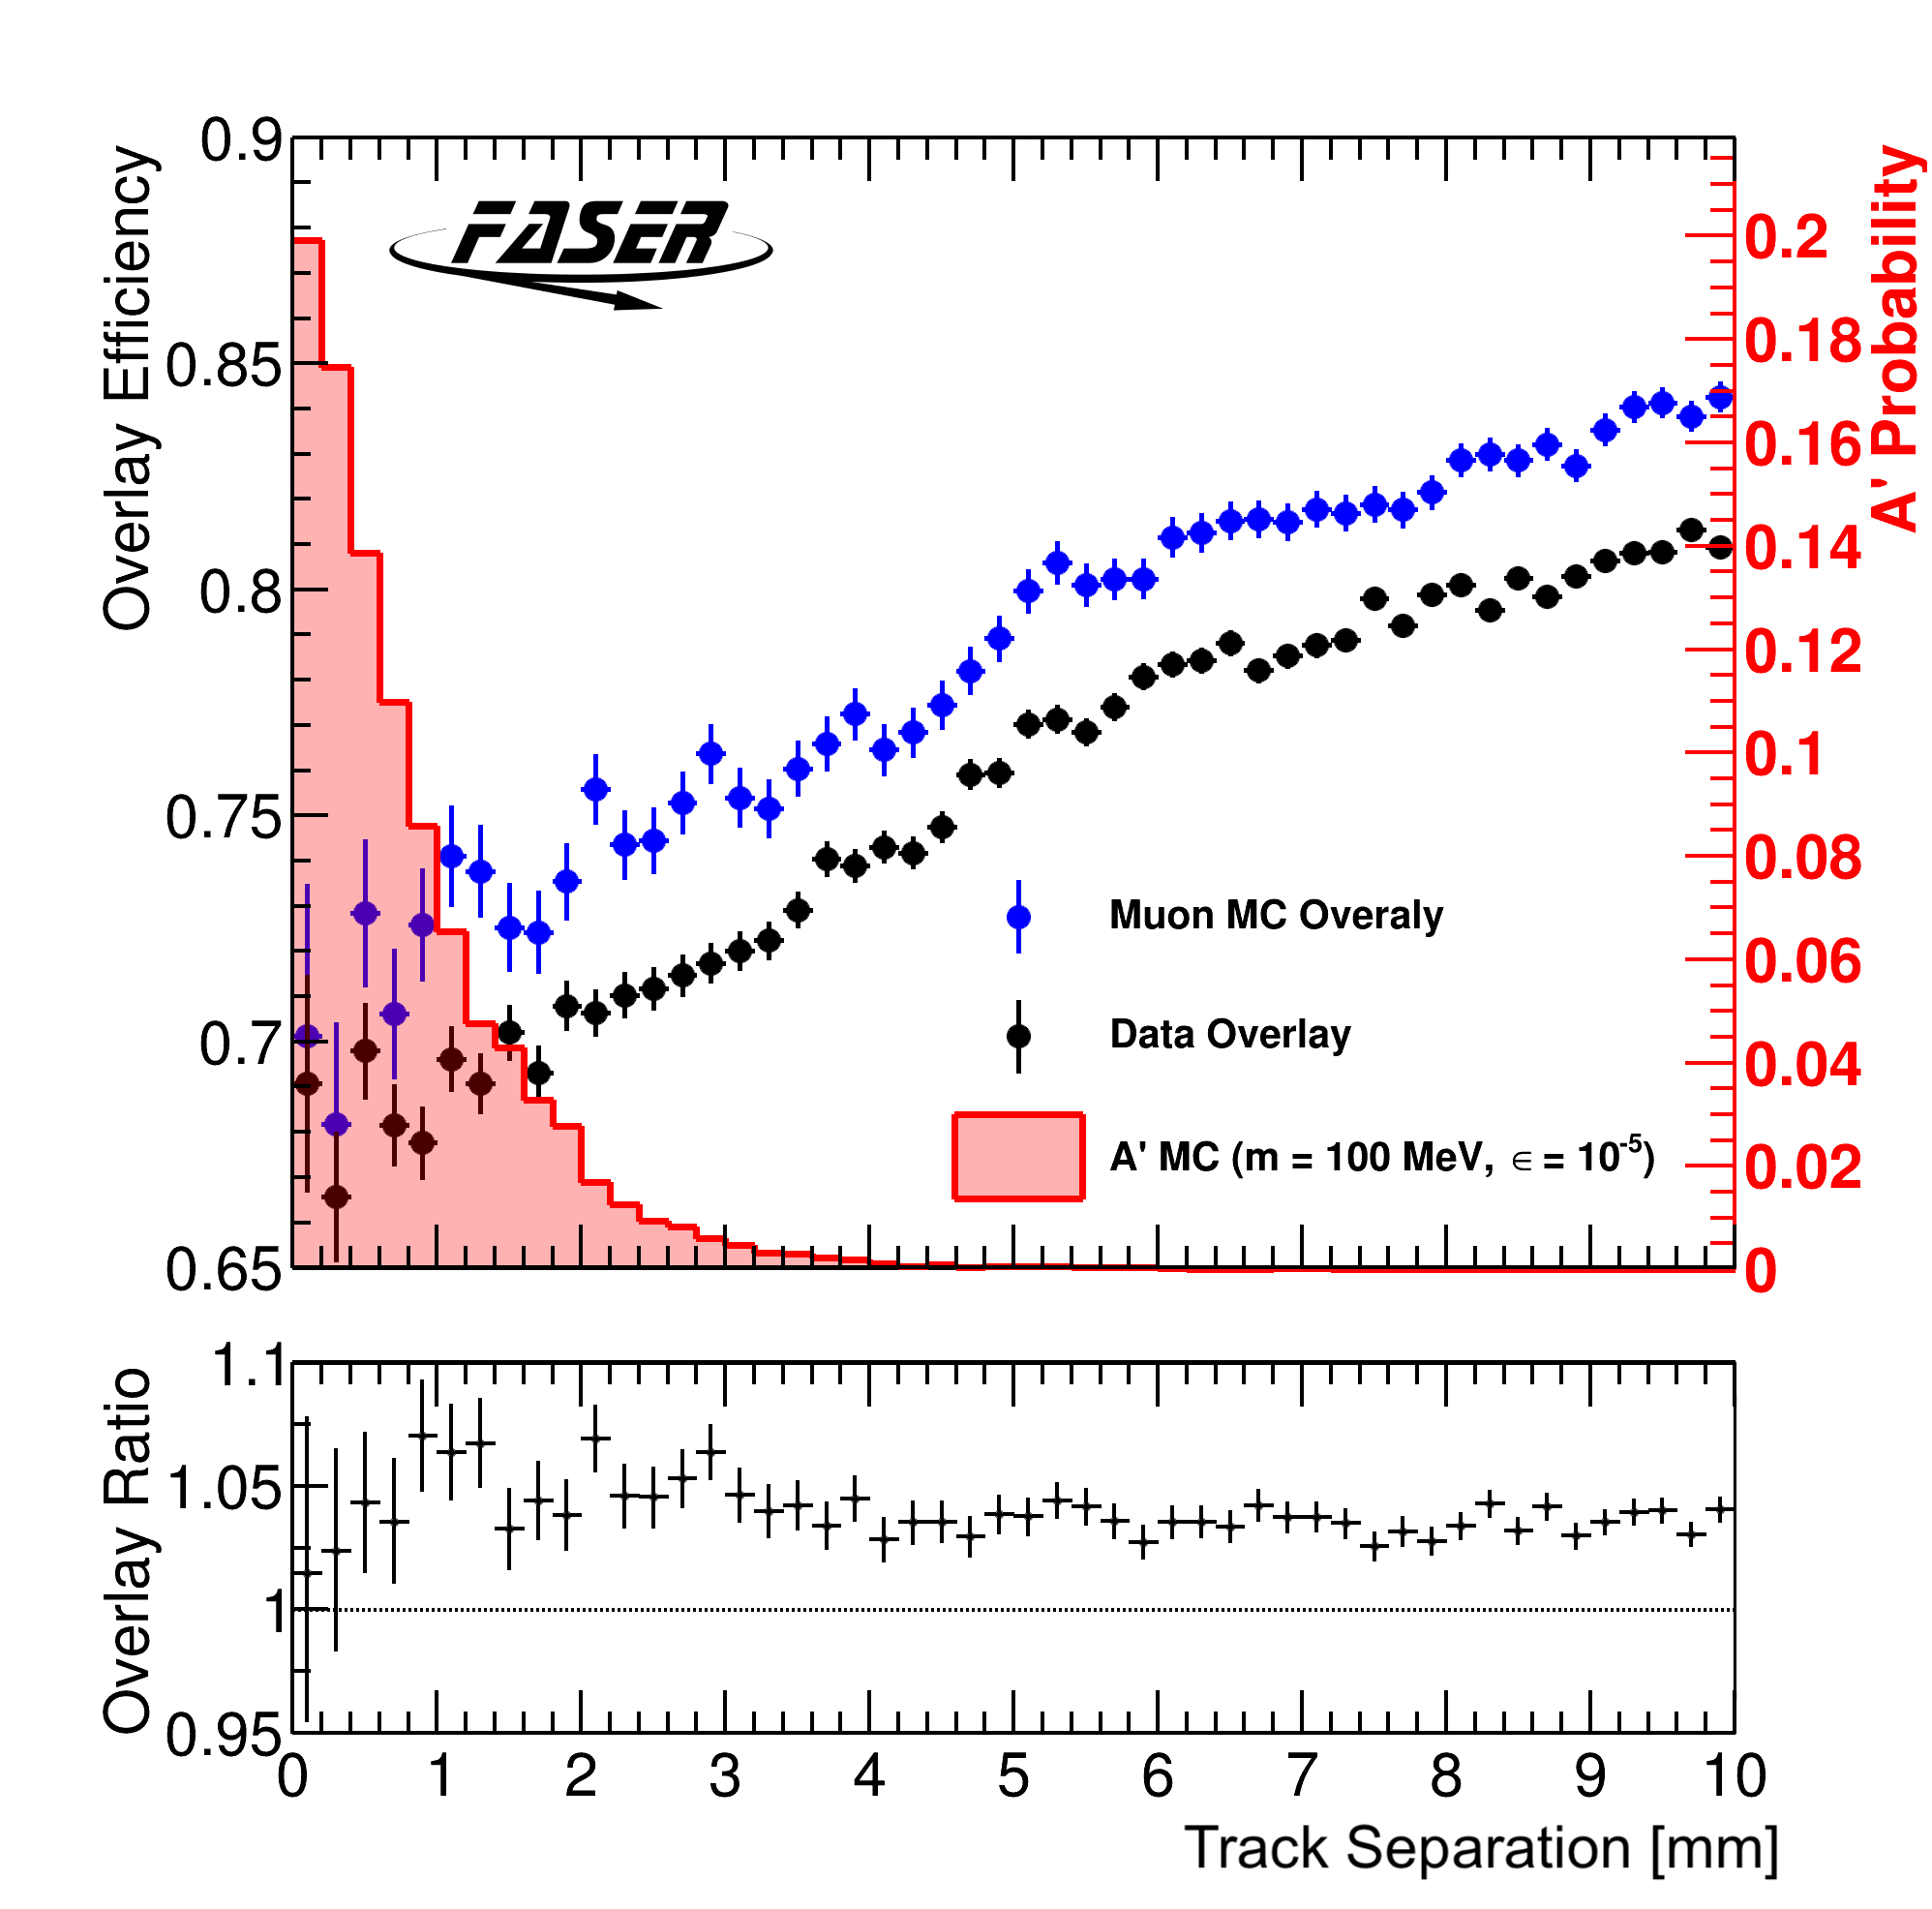
\includegraphics[width=0.8\textwidth]{assets/OverlayTracks.png}
                \caption{Overlay plot from Dark Photon Analysis}
            \end{figure}
        \end{column}
        \begin{column}{0.5 \textwidth}
            \begin{figure}
                \centering
                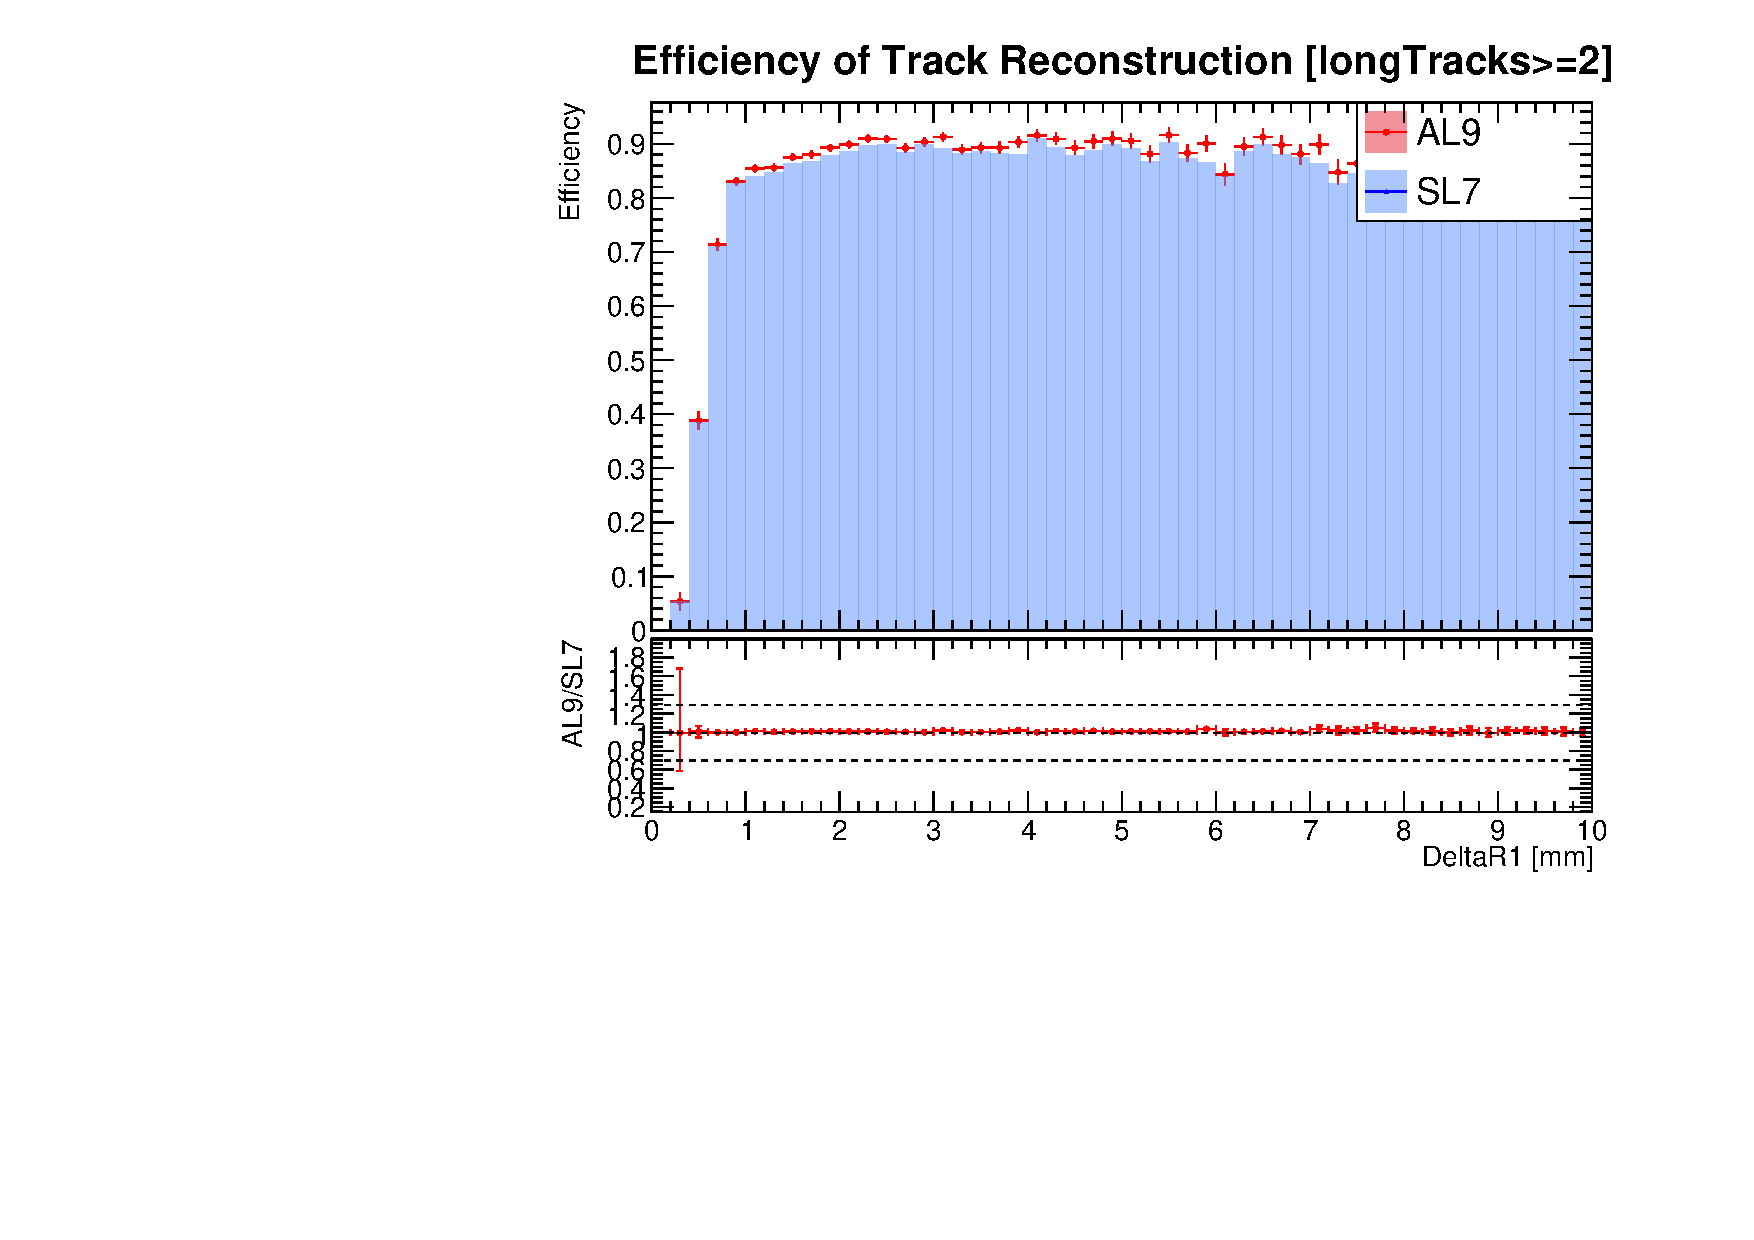
\includegraphics[width=1.1\textwidth]{assets/NEffi_greq2_DeltaR1.pdf}
                \caption{Track Efficiency ($\geq$2) as a function of distance between the tracks at the final station}
            \end{figure}
        \end{column}
    \end{columns}
    \begin{itemize}
        \item Discrepancy  with overlay studies
        \item But atleast good agreement between ALMA9 and CENTOS7
        % \item Hopefully,
    \end{itemize}
\end{frame}